\documentclass{beamer}
\usepackage{inconsolata}
\usepackage{caption}
\usepackage{color}
\usepackage{listings}
\usepackage{subfig}
\usepackage{cooltooltips}
\usepackage{hyperref}
\usepackage{perpage}
\usepackage[normalem]{ulem}
\setbeamertemplate{navigation symbols}{}%remove navigation symbols
\usepackage{listings}
\usepackage{color}
\usepackage{framed}

\definecolor{background}{RGB}{39, 40, 34}
\definecolor{string}{RGB}{230, 219, 116}
\definecolor{comment}{RGB}{117, 113, 94}
\definecolor{normal}{RGB}{248, 248, 242}
\definecolor{identifier}{RGB}{166, 226, 46}



\lstset{
  language=C,               			% choose the language of the code
  alsolanguage=Python,            			% choose the language of the code
  alsolanguage=Java,            			% choose the language of the code
  numbers=none,                   		% where to put the line-numbers
  stepnumber=1,                   		% the step between two line-numbers.        
  numbersep=5pt,                  		% how far the line-numbers are from the code
  extendedchars=true,
  numberstyle=\tiny\color{black}\ttfamily,
  backgroundcolor=\color{background},  		% choose the background color. You must add \usepackage{color}
  showspaces=false,               		% show spaces adding particular underscores
  showstringspaces=false,         		% underline spaces within strings
  showtabs=false,                 		% show tabs within strings adding particular underscores
  frame=single,
  framerule=0pt,
  tabsize=4,                      		% sets default tabsize to 2 spaces
  captionpos=n,                   		% sets the caption-position to bottom
  breaklines=true,                		% sets automatic line breaking
  breakatwhitespace=true,         		% sets if automatic breaks should only happen at whitespace
  title=\lstname,                 		% show the filename of files included with \lstinputlisting;
  basicstyle=\color{normal}\tiny\ttfamily,					% sets font style for the code
  keywordstyle=\color{magenta}\tiny\ttfamily,	% sets color for keywords
  stringstyle=\color{string}\tiny\ttfamily,		% sets color for strings
  commentstyle=\color{comment}\tiny\ttfamily,	% sets color for comments
  emph={True, False, format_string, eff_ana_bf, permute, eff_ana_btr, KeyError,
  ValueError, ZeroDivisionError},
  emphstyle=\color{identifier}\tiny\ttfamily,
  morekeywords={with, as}
}

\lstset{literate=%
   *{0}{{{\color{cyan}0}}}1
    {1}{{{\color{cyan}1}}}1
    {2}{{{\color{cyan}2}}}1
    {3}{{{\color{cyan}3}}}1
    {4}{{{\color{cyan}4}}}1
    {5}{{{\color{cyan}5}}}1
    {6}{{{\color{cyan}6}}}1
    {7}{{{\color{cyan}7}}}1
    {8}{{{\color{cyan}8}}}1
    {9}{{{\color{cyan}9}}}1
}



\newenvironment{enum}{
\begin{enumerate}
  \setlength{\itemsep}{1pt}
  \setlength{\parskip}{0pt}
  \setlength{\parsep}{0pt}
}{\end{enumerate}}

\hypersetup{
  colorlinks=true,
  urlcolor=pink,
}

\MakePerPage{footnote}

\title{Python 101}
\subtitle{Lec06 \\ Classes}
\author{thoum}

\begin{document}
\frame{\titlepage}

\begin{frame}
\frametitle{Programming up till now}
Procedure-Oriented Programming
We pass values to functions, get values, pass them to another function....
  \begin{center}
  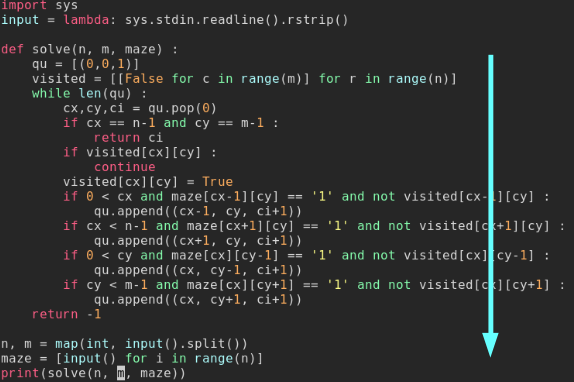
\includegraphics[width=80mm]{./code.png}
  \end{center}
\end{frame}

\begin{frame}
\frametitle{Procedure Oriented Programming}
  When programs get large, Procedure-Oriented might be \textit{too}
  complicated.\\
\end{frame}

\begin{frame}
\frametitle{Object Oriented Programming}
  Combine data and functionality in to an \textit{object}.
  View programs as object communicating with each other.
\end{frame}

\begin{frame}
\frametitle{Objects????}
  Integers are objects (of the int class).\\
  Strings are objects (of the str class).\\
  [1,2,3].sort() are their class methods, and len([1,2,3]) returns their
  internal data; length.
\end{frame}

\begin{frame}
\frametitle{Creating Classes of our own}
  We don't usually use classes so much unless we start writing bigger programs.
  The usual class tutorials force us to create boring exmaples.
  We are going to make a simple baseball game.
\end{frame}

\begin{frame}{The basis}
  There are two types of players in baseball.
  The Pitcher, and the Batter. They are all players, with their names,
  backnumbers, and team names.\\
  The Pitcher has types of balls they can throw, their speed, and avg.\\
  The batters have their hit rate, and speed.\\
  We are going to code this data using classes.
\end{frame}

\begin{frame}{The Player Class}
  This becomes the basis(or the superclass) of pitchers and batters.
  Note that all methods are denoted by the $self$ keyword.
\end{frame}

\begin{frame}{The Pitcher Class}
  The Pitcher class inherits property of the player, and have additional
  parameters like yadada.
\end{frame}

\begin{frame}{The Batter Class}
  The Pitcher class inherits property of the player, and have additional
  parameters like yadada.
\end{frame}

\begin{frame}{Creating the Pitcher}
  YAda
\end{frame}

\begin{frame}{Creating the Batters}
  YAda
\end{frame}

\begin{frame}{The computer controls the pitcher}
  pitcher.throw() $ball or strike$
\end{frame}

\begin{frame}{You control the batter}
  If hit:
    batter.hit()
  else:
    batter.stay()
  return T or F
  ball -> hit or strike -> hit.
\end{frame}

\begin{frame}{Printing the Result}
  EasyPeasy
\end{frame}

\begin{frame}{Overiding functions}
  Wondered how print([1,2,3]) -> [1,2,3] when print(3) -> 3?
  We can override the __string__(self) (__ means its internal)method to specify
  the format printed.
  For pitcher, override __string__(self): I can throw a ball at 000 km/h.
  print(pitcher)
\end{frame}

\begin{frame}{How?}
  Imagine how we use an actual Dictionary. We don't start from 'aardvark' to
  look up 'floccinaucinihilipilification'.
  We start from the F section.\\

  We have mapped 'floccinaucinihilipilification' to 'f', so that we don't have
  to compare every word; we just compare with those in the F section.
  We call this mapping $hashing$.
\end{frame}

\begin{frame}{Hashing}
  Mapping data of arbitrary size onto data of a fixed size.

  Mapping words to its first letters, mapping students to student IDs,
  mapping your socks to the colors of white, grey and black to pair them, they are all hashing.
\end{frame}

\begin{frame}{Hashing Example}
  $a=1, b=2, ...\ z=26$\\
  score of a word = $\Sigma value(c_i)\ mod\ 101$
  \begin{lstinputlisting}
    {rough_hash.py}
  \end{lstinputlisting}
\end{frame}

\begin{frame}{Hashing}
  Hashing by itself is an important topic with wide range of usage(Encryption,
  Bitcoins...), but will not go into further details.
\end{frame}

\begin{frame}{Using Dictionaries}
  \begin{lstinputlisting}
    {dict_example.py}
  \end{lstinputlisting}
\end{frame}

\begin{frame}{Using Dictionaries}
  \begin{lstinputlisting}
    {dict_example2.py}
  \end{lstinputlisting}
\end{frame}

\begin{frame}{Using Dictionaries}
  Operations on iterables(\textit{e.g.} len()) is possible on dictionaries as
  well.
\end{frame}

\begin{frame}{List vs Dictionary}
  Input: 151 pokemon's name and number.\\
  Output: Print the pokemon's number when given name.
\end{frame}

\begin{frame}{List Ver.}
  \begin{lstinputlisting}
    {poke_list.py}
  \end{lstinputlisting}
\end{frame}

\begin{frame}{Dict Ver.}
  \begin{lstinputlisting}
    {poke_dict.py}
  \end{lstinputlisting}
\end{frame}

\begin{frame}{Performance?}

\end{frame}

\begin{frame}{set}
  Unordered collection of distinct hashable objects.\\
  Used for membership, removing duplicates and so on.
\end{frame}


\begin{frame}{set examples}
  removing duplicates
  \begin{lstinputlisting}
    {./set_example.py}
  \end{lstinputlisting}
\end{frame}

\begin{frame}{set examples}
  testing membership\\
  list version: 2.978s, set version: 0.044s
  \begin{lstinputlisting}
    {./set_membership.py}
  \end{lstinputlisting}
\end{frame}

\begin{frame}{set examples}
  For other operations like union(), intersection(), difference(), look
  \href{https://docs.python.org/2/library/stdtypes.html\#set}{here}.
\end{frame}

\begin{frame}{Counter}
  Counts occurrences
  \begin{lstinputlisting}
    {./counter_example.py}
  \end{lstinputlisting}
\end{frame}

\begin{frame}{deque}
  Double Ended Queue

  Use instead of \textit{list} when inserting, popping happens at the beginning
  of the list. \textit{e.g.} keeping track of values for moving average?\\
  Insert, pop at the beginning of the list creates an overhead of
  shifting every other element to the left.\\
\end{frame}

\begin{frame}{deque vs list}
  list:3.920s, deque: 0.015s
  \begin{lstinputlisting}
    {./deque_list.py}
  \end{lstinputlisting}
\end{frame}


\begin{frame}{deque vs list}
  List outperforms deque in random access\\
  list:0.111s, deque: 3.597s
  \begin{lstinputlisting}
    {./deque_access.py}
  \end{lstinputlisting}
\end{frame}

\begin{frame}{What to use?}
  In choosing the right $thing$ to use, having a slight idea of complexity
  would help.
\end{frame}

\begin{frame}{Time/Memory Complexity}
  How long does an operation take? How much memory does it use?\\
\end{frame}

\begin{frame}{Time Complexity}
  When input size is $N$
  Some operation might take constant time. \textit{e.g.} lst[i]

  Some operation might take time proportional to N.

  \textit{e.g.} iterating over a list

  Some operation might take time proportional to $N^{2}$.

  \textit{e.g.} matrix multiplication\\

  Some operation might take time proportional to $Nlog(N)$.

  \textit{e.g.} sorting
\end{frame}

\begin{frame}{Time-Memory Tradeoff}
  Things can be sped up by using memory.
  We memorized 99dan, so it takes us constant time to answer 9*9.

  We didn't memorize(at least I didn't) every integer multiplication,
  so it takes us time to answer 938212834 * 41237.
\end{frame}

\begin{frame}{Time-Memory Tradeoff}
  In C, strlen() counts the number of letters, so it takes time proportional to the length of the string.

  In Python, len() returns an internally stored length which is updated everytime the list changes.

  There is a tradeoff between memory, and speed.
\end{frame}

\begin{frame}{Time-Memory Tradeoff}
  Python dicts uses extra memory, and hash computing time, to make
  access fast enough.

  In fact, we can think that Python itself uses more running time and memory to make coding fast enough.
\end{frame}


\end{document}
